\PassOptionsToPackage{usenames}{color}
\documentclass[11pt,letterpaper]{article}
\usepackage{etex} % remove ``No room for a new \dimen'' error

\usepackage{relsize} % relative font sizes (e.g. \smaller). must precede ACL style
\usepackage{style/naaclhlt2016}

%\naaclfinalcopy % Uncomment this line for the final submission
\def\naaclpaperid{***} %  Enter the naacl Paper ID here

% To expand the titlebox for more authors, uncomment
% below and set accordingly.
% \addtolength\titlebox{.5in}    

\usepackage[colorlinks=true,linkcolor=black,citecolor=black,filecolor=black,urlcolor=black]{hyperref}
\usepackage{natbib}
\newcommand{\citeposs}[1]{\citeauthor{#1}'s (\citeyear{#1})}

%\usepackage{times}
%\usepackage{latexsym}

\usepackage{framed}
\usepackage[boxed]{algorithm2e}
\renewcommand\AlCapFnt{\small}
\usepackage[small,bf,skip=5pt]{caption}
\usepackage{sidecap} % side captions
\usepackage{rotating}	% sideways

% Italicize subparagraph headings
\usepackage{titlesec}
\titleformat*{\subparagraph}{\itshape}
\titlespacing{\subparagraph}{%
  1em}{%              left margin
  0pt}{% space before (vertical)
  1em}%               space after (horizontal)

% Numbered Examples and lists
\usepackage{lingmacros}

\usepackage{enumitem} % customizable lists
\setitemize{noitemsep,topsep=0em,leftmargin=*}
\setenumerate{noitemsep,leftmargin=0em,itemindent=13pt,topsep=0em}
%%reduce space around captions
%\setlength{\abovecaptionskip}{1pt plus 1pt minus 1pt}
%\setlength{\belowcaptionskip}{1pt plus 1pt minus 1pt}

%\titlespacing*\section{0pt}{6pt plus 4pt minus 2pt}{4pt plus 2pt minus 2pt}
%\titlespacing*\subsection{1pt}{6pt plus 4pt minus 2pt}{0pt plus 2pt minus 2pt}
%\titlespacing*\subsubsection{1pt}{6pt plus 4pt minus 2pt}{0pt plus 2pt minus 2pt}
%\titlespacing*\paragraph{1pt}{6pt plus 4pt minus 2pt}{0pt plus 2pt minus 2pt}


\usepackage{textcomp}
% \usepackage{arabtex} % must go after xparse, if xparse is used!
%\usepackage{utf8}
% \setcode{utf8} % use UTF-8 Arabic
% \newcommand{\Ar}[1]{\RL{\novocalize #1}} % Arabic text

\usepackage{listings}

\lstset{
  basicstyle=\itshape,
  xleftmargin=3em,
  aboveskip=0pt,
  belowskip=-3pt, %-.5\baselineskip, % correct for extra paragraph break inserted after listing
  literate={->}{$\rightarrow$}{2}
           {α}{$\alpha$}{1}
           {δ}{$\delta$}{1}
           {(}{$($}{1}
           {)}{$)$}{1}
           {[}{$[$}{1}
           {]}{$]$}{1}
           {|}{$|$}{1}
           {+}{\ensuremath{^+}}{1}
           {*}{\ensuremath{^*}}{1}
}

\usepackage{amssymb}	%amsfonts,eucal,amsbsy,amsthm,amsopn
\usepackage{amsmath}

\usepackage{mathptmx}	% txfonts
\usepackage[scaled=.8]{beramono}
\usepackage[T1]{fontenc}
\usepackage[utf8x]{inputenc}

\usepackage{MnSymbol}	% must be after mathptmx

\usepackage{latexsym}

% Graphics
\usepackage{tikz}
\usetikzlibrary{arrows,positioning,calc} 



% Tables
\usepackage{array}
\usepackage{multirow}
\usepackage{booktabs} % pretty tables
\usepackage{multicol}
\usepackage{footnote}
\newcolumntype{H}{>{\setbox0=\hbox\bgroup}c<{\egroup}@{}} % hidden column

\usepackage{url}
\usepackage[usenames]{color}
\usepackage{xcolor}

% colored frame box
\newcommand{\cfbox}[2]{%
    \colorlet{currentcolor}{.}%
    {\color{#1}%
    \fbox{\color{currentcolor}#2}}%
}

\usepackage[normalem]{ulem} % \uline
\usepackage{colortbl}
\usepackage{graphicx}
\usepackage{subcaption}
%\usepackage{tikz-dependency}
%\usepackage{tikz}
%\usepackage{tree-dvips}
%\usetikzlibrary{arrows,positioning,calc} 
\usepackage{xytree}

\usepackage{xspace} % \xspace command for macros (inserts a space unless followed by punctuation)

\DeclareMathOperator*{\argmax}{arg\,max}
\DeclareMathOperator*{\argmin}{arg\,min}
\setlength\titlebox{4cm}    % Expanding the titlebox



% Author comments
\usepackage{color}
\newcommand\bmmax{0} % magic to avoid 'too many math alphabets' error
\usepackage{bm}
\definecolor{orange}{rgb}{1,0.5,0}
\definecolor{mdgreen}{rgb}{0,0.6,0}
\definecolor{mdblue}{rgb}{0,0,0.7}
\definecolor{dkblue}{rgb}{0,0,0.5}
\definecolor{dkgray}{rgb}{0.3,0.3,0.3}
\definecolor{slate}{rgb}{0.25,0.25,0.4}
\definecolor{gray}{rgb}{0.5,0.5,0.5}
\definecolor{ltgray}{rgb}{0.7,0.7,0.7}
\definecolor{purple}{rgb}{0.7,0,1.0}
\definecolor{lavender}{rgb}{0.65,0.55,1.0}

% Settings for algorithm listings
% \lstset{
%   language=Python,
%   upquote=true,
%   showstringspaces=false,
%   formfeed=\newpage,
%   tabsize=1,
%   commentstyle=\itshape\color{lavender},
%   basicstyle=\small\smaller\ttfamily,
%   morekeywords={lambda},
%   emph={upward,downward,tc},
%   emphstyle=\underbar,
%   aboveskip=0cm,
%   belowskip=-.5cm
% }
%\renewcommand{\lstlistingname}{Algorithm}


\newcommand{\ensuretext}[1]{#1}
\newcommand{\cjdmarker}{\ensuretext{\textcolor{green}{\ensuremath{^{\textsc{CJ}}_{\textsc{D}}}}}}
\newcommand{\nssmarker}{\ensuretext{\textcolor{magenta}{\ensuremath{^{\textsc{NS}}_{\textsc{S}}}}}}
\newcommand{\nasmarker}{\ensuretext{\textcolor{red}{\ensuremath{^{\textsc{NA}}_{\textsc{S}}}}}}
\newcommand{\dhmarker}{\ensuretext{\textcolor{red}{\ensuremath{^{\textsc{D}}_{\textsc{H}}}}}}
\newcommand{\lkmarker}{\ensuretext{\textcolor{blue}{\ensuremath{^{\textsc{L}}_{\textsc{K}}}}}}
\newcommand{\swswmarker}{\ensuretext{\textcolor{orange}{\ensuremath{^{\textsc{S}}_{\textsc{S}}}}}}
\newcommand{\abmarker}{\ensuretext{\textcolor{purple}{\ensuremath{^{\textsc{A}}_{\textsc{B}}}}}}
\newcommand{\mcmarker}{\ensuretext{\textcolor{dkblue}{\ensuremath{^{\textsc{M}}_{\textsc{C}}}}}}
\newcommand{\arkcomment}[3]{\ensuretext{\textcolor{#3}{[#1 #2]}}}
%\newcommand{\arkcomment}[3]{}
\newcommand{\nss}[1]{\arkcomment{\nssmarker}{#1}{magenta}}
\newcommand{\aj}[1]{\arkcomment{\cjdmarker}{#1}{green}}
\newcommand{\dirk}[1]{\arkcomment{\dhmarker}{#1}{red}}
\newcommand{\lk}[1]{\arkcomment{\lkmarker}{#1}{blue}}
\newcommand{\swsw}[1]{\arkcomment{\swswmarker}{#1}{orange}}
\newcommand{\ab}[1]{\arkcomment{\abmarker}{#1}{purple}}
\newcommand{\mc}[1]{\arkcomment{\mcmarker}{#1}{dkblue}}
\newcommand{\wts}{\mathbf{w}}
\newcommand{\g}{\mathbf{g}}
\newcommand{\f}{\mathbf{f}}
\newcommand{\x}{\mathbf{x}}
\newcommand{\y}{\mathbf{y}}
\newcommand{\overbar}[1]{\mkern 1.5mu\overline{\mkern-1.5mu#1\mkern-1.5mu}\mkern 1.5mu} % \bar is too narrow in math
\newcommand{\cost}{c}

\usepackage{nameref}
\usepackage{cleveref}

% use \S for all references to all kinds of sections, and \P to paragraphs
% (sadly, we cannot use the simpler \crefname{} macro because it would insert a space after the symbol)
\crefformat{part}{\S#2#1#3}
\crefformat{chapter}{\S#2#1#3}
\crefformat{section}{\S#2#1#3}
\crefformat{subsection}{\S#2#1#3}
\crefformat{subsubsection}{\S#2#1#3}
\crefformat{paragraph}{\P#2#1#3}
\crefformat{subparagraph}{\P#2#1#3}
%\crefmultiformat{part}{\S#2#1#3}{ and~\S#2#1#3}{, \S#2#1#3}{, and~\S#2#1#3}
%\crefmultiformat{chapter}{\S#2#1#3}{ and~\S#2#1#3}{, \S#2#1#3}{, and~\S#2#1#3}
\crefmultiformat{section}{\S#2#1#3}{ and~\S#2#1#3}{, \S#2#1#3}{, and~\S#2#1#3}
\crefmultiformat{subsection}{\S#2#1#3}{ and~\S#2#1#3}{, \S#2#1#3}{, and~\S#2#1#3}
\crefmultiformat{subsubsection}{\S#2#1#3}{ and~\S#2#1#3}{, \S#2#1#3}{, and~\S#2#1#3}
\crefmultiformat{paragraph}{\P\P#2#1#3}{ and~#2#1#3}{, #2#1#3}{, and~#2#1#3}
\crefmultiformat{subparagraph}{\P\P#2#1#3}{ and~#2#1#3}{, #2#1#3}{, and~#2#1#3}
%\crefrangeformat{part}{\mbox{\S\S#3#1#4--#5#2#6}}
%\crefrangeformat{chapter}{\mbox{\S\S#3#1#4--#5#2#6}}
\crefrangeformat{section}{\mbox{\S\S#3#1#4--#5#2#6}}
\crefrangeformat{subsection}{\mbox{\S\S#3#1#4--#5#2#6}}
\crefrangeformat{subsubsection}{\mbox{\S\S#3#1#4--#5#2#6}}
\crefrangeformat{paragraph}{\mbox{\P\P#3#1#4--#5#2#6}}
\crefrangeformat{subparagraph}{\mbox{\P\P#3#1#4--#5#2#6}}
% for \label[appsec]{...}
\crefname{part}{Part}{Parts}
\Crefname{part}{Part}{Parts}
\crefname{chapter}{ch.}{ch.}
\Crefname{chapter}{Ch.}{Ch.}
\crefname{figure}{figure}{figures}
\crefname{appsec}{appendix}{appendices}
\Crefname{appsec}{Appendix}{Appendices}
\crefname{algocf}{algorithm}{algorithms}
\Crefname{algocf}{Algorithm}{Algorithms}
\crefname{enums,enumsi}{example}{examples}
\Crefname{enums,enumsi}{Example}{Examples}
\crefname{}{example}{examples} % lingmacros \toplabel has no internal name for the kind of label
\Crefname{}{Example}{Examples}
\crefformat{enums}{(#2#1#3)}
\crefformat{enumsi}{(#2#1#3)}
\crefformat{}{(#2#1#3)}
\crefrangeformat{enums}{\mbox{(#3#1#4--#5#2#6)}}
\crefrangeformat{enumsi}{\mbox{(#3#1#4--#5#2#6)}}

\ifx\creflastconjunction\undefined%
\newcommand{\creflastconjunction}{, and\nobreakspace} % Oxford comma for lists
\else%
\renewcommand{\creflastconjunction}{, and\nobreakspace} % Oxford comma for lists
\fi%

\newcommand*{\Fullref}[1]{\hyperref[{#1}]{\Cref*{#1}: \nameref*{#1}}}
\newcommand*{\fullref}[1]{\hyperref[{#1}]{\cref*{#1}: \nameref{#1}}}
\newcommand{\fnref}[1]{footnote~\ref{#1}} % don't use \cref{} due to bug in (now out-of-date) cleveref package w.r.t. footnotes
\newcommand{\Fnref}[1]{Footnote~\ref{#1}}


% Space savers
% From http://www.eng.cam.ac.uk/help/tpl/textprocessing/squeeze.html
% \addtolength{\dbltextfloatsep}{-.5cm} % space between last top float or first bottom float and the text.
% \addtolength{\intextsep}{-.5cm} % space left on top and bottom of an in-text float.
% \addtolength{\abovedisplayskip}{-.5cm} % space before maths
% \addtolength{\belowdisplayskip}{-.5cm} % space after maths
% %\addtolength{\topsep}{-.5cm} %space between first item and preceding paragraph
%\setlength{\belowcaptionskip}{-.5cm}


% customize \paragraph spacing
% \makeatletter
% \renewcommand{\paragraph}{%
%   \@startsection{paragraph}{4}%
%   {\z@}{.2ex \@plus 1ex \@minus .2ex}{-1em}%
%   {\normalfont\normalsize\bfseries}%
% }
% \makeatother


% Special macros
\newcommand{\tg}[1]{\texttt{#1}}	% tag name
\newcommand{\sst}[1]{\textsc{#1}} % supersense category
\newcommand{\gfl}[1]{%\renewcommand\texttildelow{{\lower.74ex\hbox{\texttt{\char`\~}}}} % http://latex.knobs-dials.com/
\mbox{\textsmaller{\texttt{#1}}}}	% supersense tag symbol
%\newcommand{\lex}[1]{\textsmaller{\textsf{\textcolor{slate}{\textbf{#1}}}}}	% example lexical item 
\newcommand{\tagdef}[1]{#1\hfill} % tag definition
\newcommand{\tagt}[2]{\ensuremath{\underset{\textrm{\textlarger{\tg{#2}}}\strut}{\w{#1}\rule[-.3\baselineskip]{0pt}{0pt}}}} % tag text (a word or phrase) with an SST. (second arg is the tag)
\newcommand{\tagtt}[3]{\begin{tabular}{@{\hspace{2pt}}c@{\hspace{2pt}}} \texttt{#2}\\ #1 \\ \texttt{#3}\end{tabular}}
\newcommand{\tagts}[3]{\begin{tabular}{@{\hspace{2pt}}c@{\hspace{2pt}}} \texttt{#2\vphantom{\textlarger{Ĩ}}}\\ #1 \\ \sst{#3}\end{tabular}}
\newcommand{\tgt}[2]{\ensuremath{\underset{\text{\textlarger{#2}\strut}}{\text{#1\rule[-.3\baselineskip]{0pt}{\baselineskip}}}}} % tag text (a word or phrase, not underlined) with a label. (second arg is the label)
\newcommand{\glosst}[2]{\ensuremath{\underset{\textrm{#2}}{\textrm{#1}}}} % gloss text (a word or phrase) (second arg is the gloss)
\newcommand{\AnnA}[0]{\mbox{\textbf{Ann-A}}} % annotator A
\newcommand{\AnnB}[0]{\mbox{\textbf{Ann-B}}} % annotator B
\newcommand{\sys}[1]{\mbox{\textbf{#1}}}   % name of a system (one of our experimental conditions)
\newcommand{\dataset}[1]{\mbox{\textsc{#1}}}	% one of the datasets in our experiments
\newcommand{\datasplit}[1]{\mbox{\textbf{#1}}}	% portion one of the datasets in our experiments

\newcommand{\w}[1]{\textit{#1}}	% word
\newcommand{\lex}[1]{\textit{#1}} % lexical item
\newcommand{\tweet}[1]{\textsf{#1}}	% tweet
\newcommand{\twbank}[0]{\textsc{Tweebank}\xspace}
\newcommand{\foster}[0]{\textsc{Foster}\xspace}
\newcommand{\twparser}[0]{\textsc{Tweeboparser}\xspace}
\newcommand{\tat}[0]{\textasciitilde}
\newcommand{\backtick}[0]{\textasciigrave}

%\newcommand{\finalversion}[1]{#1}
\newcommand{\finalversion}[1]{}
\newcommand{\shortversion}[1]{}
\newcommand{\considercutting}[1]{#1}
\newcommand{\longversion}[1]{#1} % ...if only there were more space...

\hyphenation{WordNet}
\hyphenation{WordNets}
\hyphenation{VerbNet}
\hyphenation{FrameNet}
\hyphenation{SemCor}
\hyphenation{SemEval}
\hyphenation{PennConverter}
\hyphenation{TurboParser}
\hyphenation{Tweebo-parser}
\hyphenation{Twee-bank}
\hyphenation{an-aly-sis}
\hyphenation{an-aly-ses}
\hyphenation{news-text}
\hyphenation{base-line}
\hyphenation{de-ve-lop-ed}
\hyphenation{comb-over}


\title{SemEval-2016 Task~10:\\ Detecting Minimal Semantic Units and their Meanings (DiMSUM)}

\author{
Nathan Schneider \\
		School of Informatics\\
	   	University of Edinburgh\\
	    Edinburgh, UK\\
	    {\tt nschneid@inf.ed.ac.uk} \And
Dirk Hovy \quad Anders Johannsen\\
Center for Language Technology\\
University of Cophenhagen\\
Copenhagen, Denmark\\
{\tt \{krx628,ajohannsen\}@hum.ku.dk} \And
Marine Carpuat\\
Computer Science Dept.\\
University of Maryland\\
College Park, Maryland, USA\\
{\tt marine@cs.umd.edu}}


\date{}

\begin{document}
% \nss{Note: this document uses natbib rather than the standard ACL bib macros: 
% According to \citet{baldwin-10}, statistical association measures 
% are one technique for extracting MWE types \citep[cf.][\emph{inter alia}]{pecina-10}.}
\naaclfinalcopy % show authors
\maketitle
\global\naaclfinalfalse % turn on header/line numbers for review

\begin{abstract}\nss{TODO: rewrite}
We propose a SemEval~2016 Shared Task 
of analyzing the lexical semantics of English sentences 
in a broad-coverage fashion. 
The task formulation consists of two closely related steps which can be performed jointly:
(a)~chunking tokens within sentences into \textbf{multiword expressions}, and 
(b)~assigning coarse \textbf{supersense} labels to all noun and verb expressions. 
The evaluation will build upon recently annotated datasets in two social web genres.
\longversion{We expect that the task formulation will foster engagement across 
multiple subcommunities of computational semantics, 
and facilitate empirical comparison of methodologically diverse systems.}
\end{abstract}

\section{Introduction}\label{sec:intro}

Broad-coverage NLP techniques have, thanks in part to previous SemEval shared tasks, 
become mainstream for several aspects of language---including morphology, syntax, 
and some areas of semantics (notably, named entity recognition, %\nss{2002/2003}
semantic role labeling, %\nss{2004/2005/2008/2009} 
and coreference resolution). %\nss{2011/2012}
Explicit analysis of lexical semantics, by contrast, has been more difficult to scale 
to broad coverage. %\nss{need to say something about purely unsupervised distributional approaches?} 
This might be attributable to the dominant paradigm of word sense disambiguation 
with lexical resources such as WordNet \citep{wordnet}.
The fine-grained sense inventories in these resources 
are difficult to annotate in corpora, result in considerable data sparseness, 
and do not readily generalize to out-of-vocabulary words.
The main corpus that is annotated with WordNet senses, 
SemCor \citep{semcor}, reflects several genres of edited text, but
unfortunately, expanding the annotations to new genres---such as social web text 
or transcribed speech---would be quite expensive.
This limits the applicability of SemCor-based NLP tools 
and restricts opportunities for linguistic studies of lexical semantics in corpora.

%Here we describe the linguistic representation, annotated data, evaluation procedure, and results.
%aimed at establishing a broad-coverage paradigm for lexical semantic analysis, 
%one which we believe is suitable for a SemEval shared task. 
This task aims to establish a broad-coverage paradigm for lexical semantic analysis.
We motivate the two components of the lexical representation---multiword expressions 
and supersenses---before delving into the data, evaluation, and results.

% \nss{motivation: lexical semantic analysis of MWEs and supersenses in English. 
% semantics is a hot topic.
% highlights: (a) broad-coverage---not too far from NER; hopefully avoid some of the limitations of traditional WSD. 
% (b) robust to domain---in fact, evaluation consists of 2 social web domains.
% (c) potential to benefit from many different NLP techniques, including sequence tagging/chunking, 
% parsing, distributional word representations, language models, 
% use of language resources such as WordNet, (other buzzwords?)}

\textbf{Multiword expressions.} 
For the most part, contemporary approaches to English syntactic and semantic analysis
treat space-separated words as the basic units of structure. 
%It has even been suggested that dependency syntax, for example, 
%offers a good approximation of semantic structure.
But for sentences with noncompositional or idiosyncratic expressions, this fails to reflect 
the basic units of meaning. For example, consider:
%\begin{enumerate}[leftmargin=*,labelsep=2em,label=(\arabic*),before=\raggedright]
\begin{itemize}[labelindent=2em]
\item[(1)] The staff leaves a lot to be desired .
\item[(2)] \raggedright I googled restaurants in the area and Fuji Sushi came up and reviews were great so I made a carry out order of : L 17 .
\end{itemize}
In these sentences, \lex{a lot}, \lex{leaves\ldots to be desired}, 
\lex{Fuji Sushi}, \lex{came up}, \lex{made\ldots order}, and \lex{carry out}
are all \textbf{multiword expressions} (MWEs) 
in that their combined meanings can be thought of as ``prepackaged'' 
in a single lexical expression that happens to be written with spaces.\footnote{This is not to say that MWEs cannot have ``normal'' 
syntactic structure; some are more fixed in their form while others are quite flexible. 
For instance, \lex{make\ldots order} can be passivized just like canonical transitive verb phrases.}
MWEs such as these (and many other flavors) have attracted a great deal of attention 
within computational semantics; see \citet{baldwin-10} for a review.
\Citet{schneider-14-corpus} introduced an English corpus resource annotated for heterogenous MWEs, 
suitable for training and evaluating general-purpose MWE identification systems \citep{schneider-14}.
Prior to that, 
most MWE evaluations had assumed 
particular languages and constructions \citep[recently:][]{constant-11,green-12,ramisch-12,vincze-13},
though the corpus and identification system of \citet{vincze-11} targets several kinds of MWEs.

Importantly, the MWEs in \citeposs{schneider-14-corpus} corpus are not required to be contiguous, 
but may contain \textbf{gaps} (viz.: \lex{made\ldots order}). 
Moreover, the MWEs are qualitatively labeled as either \textbf{strong} 
(somewhat noncompositional---e.g., proper names and idioms) 
or \textbf{weak} (compositional but statistically idiomatic, as in \lex{highly recommend(ed)}). 
For simplicity, we do not include weak MWEs in the task data; 
all annotated MWEs are implicitly strong.

\textbf{Supersenses.}
% \longversion{
% Ideally, a lexical semantic representation would apply to a large number of word types 
% while being sufficiently fine-grained to disambiguate words with multiple meanings. 
% %A representation represents good coverage if it provides labels for most word classes. 
% %It offers sufficient distinction if it allows one to group words into clusters, 
% %in order to make generalizations about semantic classes. 
% A good meaning representation should also group together related meanings from different words. 
% %is typically anti-correlated with the number of available labels.
% These ideals are sometimes at odds:  \nss{\ldots}
% 
% Popular representations are named-entity tags and WordNet \citep{wordnet} word senses. 
% However, both present a problem in one of the desired aspects. 
% Named entity tags have a reasonable distinction, and are thus frequently used to find entities of a certain type. 
% However, as the name already suggests, this representation is limited to (proper) nouns, and even though high-coverage gazetteers can be found for named entity recognition, the task has thus inherently poor coverage. 
% Word senses, on the other hand, cover all content word classes. 
% However, they are lemma-specific (i.e., sense number two of \emph{house} and \emph{building} are not the same), 
% and do not allow for generalization to larger groups.\nss{not true of WordNet, because the hierarchy allows generalization. 
% I think the problems with the WordNet-style approach are (a)~it is hard to agree on/annotate with fine-grained senses, 
% and (b)~it is hard to extend the lexicon to cover OOV words that might occur in new domains (let alone other languages).}
% }
As noted above, relying on a WordNet-like lexicon as an inventory of fine-grained, lexicalized senses 
creates problems for scalability and extensibility to new domains and languages. 
Named entity recognition (NER), which is formulated in terms of (a usually small number of) delexicalized coarse-grained classes, 
does not suffer from these problems. However, because these classes are only designed to apply to named entities, 
they provide far from complete coverage of lexical items in a corpus.

Noun and verb \textbf{supersenses}
offer a compromise approach: they can be seen as generalizing 
named entity classes to cover all nouns (with 26~classes) as well as verbs (15~classes). 
The inventory, \cref{tbl:supersenses}, originates with the top-level organization of Princeton WordNet,
but can be applied directly to annotate new data---including out-of-vocabulary words 
in English or other languages \citep{schneider-12,johannsen-14}. 
Following the lead of NER, techniques for supersense tagging have generally used statistical sequence models 
and have been evaluated in English, Chinese, and Arabic.\footnote{Evaluations used 
English SemCor \citep{ciaramita-06,paas-09}, 
English-Italian MultiSemCor \citep{picca-08,picca-09,attardi-10}, 
the Italian Syntactic-Semantic Treebank and Italian Wikipedia \citep{attardi-10,rossi-13}, 
Chinese Cilin \citep{qiu-11},  
and Arabic Wikipedia \citep{schneider-13}.}
In addition to providing human-interpretable high-level clustering information, 
features based on supersenses have been exploited in downstream semantics tasks\longversion{ 
such as preposition sense disambiguation, noun compound interpretation, and metaphor detection} 
\citep{ye-07,tratz-10,tsvetkov-13}. 

\begin{table}\centering\small
\resizebox{ \columnwidth }{!}{
\begin{tabular}{>{\sst\bgroup}l<{\egroup}>{\sst\bgroup}l<{\egroup}>{\sst\bgroup}l<{\egroup}}
n:Tops	&	n:object	&	v:cognition\\
n:act	&	n:person	&	v:communication\\
n:animal	&	n:phenomenon	&	v:competition\\
n:artifact	&	n:plant	&	v:consumption\\
n:attribute	&	n:possession	&	v:contact\\
n:body	&	n:process	&	v:creation\\
n:cognition	&	n:quantity	&	v:emotion\\
n:communication	&	n:relation	&	v:motion\\
n:event	&	n:shape	&	v:perception\\
n:feeling	&	n:state	&	v:possession\\
n:food	&	n:substance	&	v:social\\
n:group	&	n:time	&	v:stative\\
\cline{2-2}
n:location	&	v:body	&	v:weather\\
n:motive	&	v:change	&	
\end{tabular}
}% resize
\caption{The 41 noun and verb supersenses in WordNet.
WordNet supersenses for adjectives and adverbs nominally exist, 
but are based on morphosyntactic rather than semantic properties.  
There is, however, recent work on developing a taxonomy for English adjective supersenses \citep{tsvetkov-14}.}
\label{tbl:supersenses}
\end{table}

% \longversion{
% The \textbf{supersense} categories for nouns and verbs, \cref{tbl:supersenses},
% are also derived from WordNet, but represent a higher level in the taxonomy. 
% They originated from a higher-level clustering of nouns and verbs into groups, 
% and thus have good coverage.\footnote{Supersenses for adjectives and adverbs nominally exist, 
% but are based on morphosyntactic rather than semantic properties. 
% There is, however, recent work on developing a taxonomy for English adjective supersenses \citep{tsvetkov-14}.}
% Since they group individual word senses into larger groups, they allow for distinction beyond the lemma level, 
% i.e., they assign the same supersense to words with different word senses. Supersenses thus provide 
% human-interpretable high-level clustering information, and have mostly been used as features in other tasks, 
% such as preposition sense disambiguation, noun compound interpretation, and metaphor detection 
% \cite{Ye:Baldwin:2007,Tratz:Hovy:2010,Tsvetkov:ea:2013}. 
% 
% The task of supersense tagging was first introduced by \citep{Ciaramita:Altun:2006EMNLP}, 
% who used 5-fold cross validation on {\sc SemCor} to evaluate their model (structured 1st order discriminative). 
% Their evaluation also included a held-out development set on each fold that was used to estimate the number of epochs 
% and additional training data containing only verbs. Their overall $F_1$ score on {\sc SemCor} was 77.1.
% Reichartz and Paa\ss{} \citep{Reichartz:Paass:2008ECMLPKDD,Paass:Reichartz:2009SIAM} 
% reached an $F_1$ score of 80.2, using CRFs and additional features.
% 
% There has been relatively little recent work on supersense tagging, and to the best of our knowledge, all of it has been mostly limited to standard English\footnote{With few exceptions such as \cite{schneider-12,schneider-13}.} ({\sc SemCor} and {\sc SensEval}). We are not aware of any previous work on word sense disambiguation for Twitter. Our hope is that this task makes the problem more attractive to a wider audience to reach more languages and domains.
% }


\textbf{Relationship between MWEs and supersenses.}
In our view, the representation of MWEs and supersenses ought to be tightly coupled:
idiomatic combinations (MWEs) are best supersense-tagged holistically,
and this supersense category will often not be one that is normally expected based on the individual words.
For example, \lex{spill the beans} in its literal interpretation
would receive supersenses \sst{v:contact} and \sst{n:food},
whereas the idiomatic interpretation meaning `divulge a secret' is represented as
an MWE holistically tagged as \sst{v:communication}.
\Citet{schneider-15} develops this idea at length, and provides a web reviews dataset
with the integrated annotation. Here, we have expanded the paradigm to additional domains
and coordinated a controlled comparison of several systems.

\textbf{Summary.}
To date, many of the analysis problems in computational lexical semantics are niche topics.
Following \citet{schneider-15}, which integrates broad-coverage MWE identification together with supersense tagging (\cref{sec:rep}),
this shared task delivers a benchmark English dataset from several nontraditional domains (\cref{sec:data});
establishes objective, controlled evaluation procedures (\cref{sec:eval});
and compares \nss{diverse? }systems (\cref{sec:results}).\nss{results, in a nutshell}
Though our dataset is limited to English, the representation
should in principle work for other languages.
%and to foster cross-pollination between different subcommunities.

% \nss{encourage creativity of solutions}
% Semantic analysis is a powerful and promising topic, but it has been largely confined to news text, 
% i.e., standardized text written mostly in English. 
% By including a relatively new and heterogeneous domain like Twitter in the data, 
% we want to encourage creative approaches that go beyond the tried and true newswire-trained approach, 
% and open the community to wider applications. 

% This task would capitalize on current enthusiasm for semantics in NLP, 
% providing a testbed for a wide variety of technical approaches---these could include 
% linguistic feature engineering; comparing sequence models to hierarchical parsing models, or their combination 
% with joint decoding \citep{le_roux-14}; domain adaptation \citep{johannsen-14}; 
% type supervision; word clustering\slash representation learning \citep{grave-13}; 
% collocation extraction \citep{pecina-10,ramisch-12}; 
% language modeling; or other methods that exploit additional resources.

% This is a new task. 
% We believe it will attract strong participation from researchers in lexical semantics, 
% structured prediction, (semi)supervised learning, domain adaptation, and social media NLP. 
% To gauge interest, we reached out informally to a number of leaders in the field, 
% asking for feedback on the idea. Several of them have indicated that they consider this 
% a worthwhile task and will consider participating if it is accepted.
% As a rough estimate, we think it would attract participation from about 20~teams.
% If it is accepted, we will publicize the task widely in order to recruit as much participation as possible.

Beyond the results presented below, we hope 
the data and findings from this task will foster cross-pollination between different subcommunities 
and serve as a framework for integrating lexical semantics in NLP applications. 
E.g., until recently, it was unclear whether word sense disambiguation could contribute to applications 
such as machine translation \citep{carpuat-05,resnik-06}; 
subsequent work found that leveraging WSD predictions in MT required 
reformulating the task to exploit the internals of an MT system
%translations in a second language replaced abstract word senses, 
%and the single-word disambiguation targets were replaced by the multiword phrases used 
%by translation systems 
\citep{chan-07,carpuat-07,lefever-10}. 
In light of the lessons of these approaches, this task moves away 
from fine-grained sense inventories and lexicalized annotation, 
while defining a more general representation that can be useful 
for many NLP applications beyond machine translation.

\section{Representation}\label{sec:rep}

\begin{figure}\centering\small
%I highly~recommend_ Garage_Pros _to my friends .  
%"labels": {"8": ["friends", "GROUP"], "3": ["recommend", "communication"], "4": ["Garage", "GROUP"]}, "_": [[3, 6], [4, 5]], "words": [["I", "PRP"], ["highly", "RB"], ["recommend", "VBP"], ["Garage", "NNP"], ["Pros", "NNPS"], ["to", "IN"], ["my", "PRP$"], ["friends", "NNS"], [".", "."]], "~": [[2, 3, 6]]}
\begin{tikzpicture}[baseline={($(current bounding box.center)+(0,-0.5ex)$)}, node distance=0cm, auto,]
 \node[inner sep=0cm]                                  (n1) {\tagts{The}{O}{}};
 \node[inner sep=0cm,above right=0pt of n1.south east] (n2) {\tagts{staff}{O}{\textsc{n.group}}};
 \node[inner sep=0cm,above right=0pt of n2.south east] (n3) {\tagts{leaves}{\color{red}B}{\color{red}\textsc{v.cognition}}};
 \node[inner sep=0cm,above right=0pt of n3.south east] (n4) {\tagts{a}{\color{blue}b}{}};
 \node[inner sep=0cm,above right=0pt of n4.south east] (n5) {\tagts{lot}{\color{blue}i}{}};
 \node[inner sep=0cm,above right=0pt of n5.south east] (n6) {\tagts{to}{\color{red}I}{}};
%\path[-,thick,dotted, bend left=30] (n2.north) edge (n3.north); 
\path[-,thick,red, bend left=20] (n3.north) edge (n6.north);
 \path[-,thick,blue, bend left=30] (n4.north) edge (n5.north);
 \node[inner sep=0cm,above right=0pt of n6.south east] (n7) {\tagts{be}{\color{red}I}{}};
 \node[inner sep=0cm,above right=0pt of n7.south east] (n8) {\tagts{desired}{\color{red}I}{}};
\path[-,thick,red, bend left=30] (n6.north) edge (n7.north);
\path[-,thick,red, bend left=30] (n7.north) edge (n8.north);
 \node[inner sep=0cm,above right=0pt of n8.south east] (n9) {\tagts{.}{O}{}};
\end{tikzpicture}
\caption{Illustration of the target representation. MWE positional markers are shown above the sentence 
and noun and verb supersenses below the sentence. 
Links illustrate the behavior of the MWE tags.
The supersense labeling must respect the MWEs; thus, \sst{v.cognition} 
applies to a four-word unit---\emph{to}, \emph{be}, and \emph{desired} 
must not receive separate supersenses.}
\label{fig:ex1}
\end{figure}

% ewtb.r.055976.1 The staff leaves_ a_lot _to_be_desired .
% ewtb.r.389298.4 I highly~recommend_ Garage_Pros _to my friends .  
%"labels": {"8": ["friends", "GROUP"], "3": ["recommend", "communication"], "4": ["Garage", "GROUP"]}, "_": [[3, 6], [4, 5]], "words": [["I", "PRP"], ["highly", "RB"], ["recommend", "VBP"], ["Garage", "NNP"], ["Pros", "NNPS"], ["to", "IN"], ["my", "PRP$"], ["friends", "NNS"], [".", "."]], "~": [[2, 3, 6]]}
% ewtb.r.329991.1 I googled restaurants in the area and Fuji_Sushi came_up and reviews were great so I made_ a carry_out _order of : L 17 .       {"labels": {"2": ["googled", "communication"], "3": ["restaurants", "GROUP"], "6": ["area", "LOCATION"], "8": ["Fuji", "GROUP"], "10": ["came", "communication"], "13": ["reviews", "COMMUNICATION"], "14": ["were", "stative"], "18": ["made", "communication"], "20": ["carry", "possession"]}, "_": [[8, 9], [10, 11], [18, 22], [20, 21]], "words": [["I", "PRP"], ["googled", "VBD"], ["restaurants", "NNS"], ["in", "IN"], ["the", "DT"], ["area", "NN"], ["and", "CC"], ["Fuji", "NNP"], ["Sushi", "NNP"], ["came", "VBD"], ["up", "RB"], ["and", "CC"], ["reviews", "NNS"], ["were", "VBD"], ["great", "JJ"], ["so", "RB"], ["I", "PRP"], ["made", "VBD"], ["a", "DT"], ["carry", "VB"], ["out", "RP"], ["order", "NN"], ["of", "IN"], [":", ":"], ["L", "$"], ["17", "CD"], [".", "."]], "~": []}


\begin{table*}[t]\small\centering
\begin{tabular}{@{}>{\textsc\bgroup}l<{\egroup}@{~~}r@{~~}r@{~~}c@{~~}|l@{~~}r@{~~}c@{~~}>{\smaller}Hl@{~~}r@{~~}c@{~~}>{\smaller}H@{}}
\multicolumn{4}{c}{\textbf{MWE}} & \multicolumn{4}{c}{\textbf{Noun}} & \multicolumn{4}{c}{\textbf{Verb}} \\
\cmidrule(r){1-4}\cmidrule(lr){5-8}\cmidrule(l){9-12}

% adv\_prep &                       25 &      1 & \lex{even~though}
%27 & V\_A &                       19 &      6 & \lex{make~sure} \\
%28 & V\_P\_N &                     14 &      6 & \lex{put~at~ease} \\
%29 & \#\_N &                       20 &      \phantom{0}& 5~star:~9\quad 2~star:~2\quad 800~number:~1\quad one~bit:~1\quad ten~star:~1\quad 360~restraunt:~1\quad \\
%30 & N\_A &                       18 &      \phantom{0}& year~old:~9\quad month~old:~3\quad years~old:~2\quad cost~effective:~1\quad lightning~fast:~1\quad \\


n\_n &                      331 &      1 & \lex{customer~service}
	& \sst{group} & 1469 & \lex{place} & 6 &         \sst{stative} & 2922 & \lex{is} & 1 \\
pn\_pn &                      325 &      1 & \lex{santa~fe} 
	& \sst{person} & 1202 & \lex{people} & 1 &        \sst{cognition} & 1093 & \lex{know} & 4 \\
v\_prep &                      217 &     44 & \lex{work~with}
	& \sst{artifact} & 971 & \lex{car} & 2 &      \sst{communication} & 974 & \lex{recommend} & 2 \\
v\_part &                      149 &     42 & \lex{pick~up} 
	& \sst{cognition} & 771 & \lex{way} & 4 &    \sst{social} & 944 & \lex{use} & 5 \\
v\_n &                       31 &    107 & \lex{take~time}
	& \sst{food} & 766 & \lex{food} & 21 &         \sst{motion} & 602 & \lex{go} & 6 \\
adj\_n &                      133 &      3 & \lex{front~desk}
	& \sst{act} & 700 & \lex{service} & 3 &          \sst{possession} & 309 & \lex{pay} & 7 \\
v\_adv &                      103 &     30 & \lex{come~in}
	& \sst{location} & 638 & \lex{area} & 8 &     \sst{change} & 274 & \lex{fix} & 3 \\
det\_n &                       83 &      1 & \lex{a~lot}
	& \sst{time} & 530 & \lex{day} & 9 &         \sst{emotion} & 249 & \lex{love} & 11 \\
prep\_n &                       67 &      8 & \lex{on~time}
	& \sst{event} & 431 & \lex{experience} & 14 &       \sst{perception} & 143 & \lex{see} & 9 \\
adv\_adv &                       72 &      1 & \lex{at~least}
	& \sst{communication} & 417 & \lex{review} & 5 &   \sst{consumption} & 93 & \lex{have} & 12 \\
v\_det\_n &                     46 &     21 & \lex{take~the~time}
	& \sst{possession} & 339 & \lex{price} & 16 &   \sst{body} & 82 & \lex{get\ldots done} & 13 \\
v\tat n &           7 &     56 & \lex{do~job}
	& \sst{attribute} & 205 & \lex{quality} & 7 &     \sst{creation} & 64 & \lex{cook} & 10 \\
pn\_pn\_pn &             63 &     \phantom{0}& \lex{home~delivery~service}
	& \sst{quantity} & 102 & \lex{amount} & 13 &      \sst{contact} & 46 & \lex{put} & 8 \\
adv\tat v &                     49 &      \phantom{0}& \it \lex{highly~recommend}
	& \sst{animal} & 88 & \lex{dog} & 18 &         \sst{competition} & 11 & \lex{win} & 14 \\
prep\_det\_n &                     33 &      6 & \lex{over~the~phone}
	& \sst{body} & 87 & \lex{hair} & 11 &          \sst{weather} & 0 & --- & 15 \\
\cline{9-12}
adj\_prep &                       39 &      \phantom{0}& \lex{pleased~with}
	& \sst{state} & 56 & \lex{pain}            & 10 & \textbf{\smaller[.5] all 15 VSSTs} & \textbf{7806} & \\
prep\_prep &                       39 &      \phantom{0}& \lex{out~of}
	& \sst{natural object} & 54 & \lex{flower} & 15 & \textsmaller[.5]{auxiliary verbs} & 1191 & \lex{have} &  \\
v\_pron &                       38 &      \phantom{0}& \lex{thank~you}
	& \sst{relation} & 35 & \lex{portion} & 19 &  \\
v\_v &                        8 &     30 & \lex{get~do}
	& \sst{substance} & 34 & \lex{oil} & 12     &  \\
n\tat n &                    34 &      1 & \lex{channel~guide}
	& \sst{feeling} & 34 & \lex{discomfort} & 20 &  \\
adj\tat n &                    31 &      \phantom{0}& \lex{hidden~gem}
	& \sst{process} & 28 & \lex{process} & 22 &     \\
v\_n\_prep &                     16 &     15 & \lex{take~care~of}
	& \sst{motive} & 25 & \lex{reason} & 25 & \\
n\_v &                       18 &     10 & \lex{mind~blow}
	& \sst{phenomenon} & 23 & \lex{result} & 17 & \\
pn\_poss &                       28 &      \phantom{0}& \lex{bj~s}
	& \sst{shape} & 6 & \lex{square} & 24 & \\
det\_adj &                       28 &      \phantom{0}& \lex{a~few}
	 & \sst{plant} & 5 & \lex{tree} & 23 & \\
\multicolumn{4}{c|}{\textsmaller{\ldots~435 additional patterns~\ldots}} % 460-25
	& \sst{other} & 2 & \lex{stuff} & 26 & \\
\cline{1-4}\cline{5-8}
\multicolumn{1}{@{}l}{\textbf{\smaller[.5] all MWEs}} & \textbf{2948} & \textbf{535} & \textbf{= 3483 total instances}
 & \textbf{\smaller[.5] all 26 NSSTs} & \textbf{9018} 
\end{tabular}

\caption{Top MWE patterns along with frequency-ranked noun and verb supersense tagsets from the \textsc{Reviews} corpus. 
The last column of each entry shows the most frequent lexical item (lemma sequence) of the class.
MWE patterns are strong (\_) or weak (\tat) sequences of coarse parts of speech. (\textsc{pn} stands for ``proper noun.'')
Contiguous and gappy MWE counts are distinguished: e.g.,~78\% of instances of the \textsc{v\_n} pattern 
contain a gap (with one or more intervening words).
Supersense counts do not distinguish single-word vs.~multiword expressions.
}
\label{tbl:reviews}
\end{table*}

\longversion{To facilitate (but not require) joint sequence modeling, 
the lexical semantic}\shortversion{The} analysis for each sentence will be represented as 
a sequence of joint MWE+supersense tags. \Cref{fig:ex1} illustrates 
the MWE part above the sentence and the supersense part below\longversion{ the sentence}; 
in practice, these will be hyphenated into a single tag per token.

The MWE portion is a BIO-style \citep{ramshaw-95} 
positional marker. Of the schemes discussed by \citet{schneider-14}, 
we adopt the 6-tag scheme, which uses case to allow gaps in an MWE (lowercase tag variants mark 
tokens within a gap).
The positions are thus \texttt{O}, \texttt{o}, \texttt{B}, \texttt{b},
\texttt{I}, \texttt{i}.
Systems are expected to ensure that the full tag sequence for a sentence is valid: 
global validity can be enforced with first-order constraints 
to prohibit invalid bigrams such as \texttt{O~I} and \texttt{b~I} (see \citealp{schneider-14} for details).

Because strong MWEs receive a supersense as a unit (if at all), 
\texttt{I} and \texttt{i} are never conjoined with a supersense label.
\texttt{O} or \texttt{o} indicates that the token is not part of any MWE, 
but many such tokens do bear a noun or verb supersense.
%\longversion{Of course, the supersenses in this task only cover noun and verb expressions, 
%so plain \texttt{O} will be frequent, as will plain \texttt{B} and \texttt{Ī} for (e.g.) PP idioms.}

This task uses a CoNLL-style main \textbf{file format}
consisting of one line per token, each line having 9~tab-delimited columns, 
as explained in \cref{fig:tagsformat} in the annex.
Scripts to convert to and from the \texttt{.sst} format, which displays one sentence per line 
and contains annotations in a JSON data structure, are provided as well.
\longversion{All file formats are UTF-8 encoded.}



\section{Data}\label{sec:data}

The task built upon two existing datasets of social web text, which were 
harmonized to form the training data. Four new samples from three domains 
were annotated from scratch to form the test set.
The train and test sets are summarized in \cref{tbl:datasets}. 
%These capture two genres of social web text:

\begin{table}
\caption{\nss{Summary of component datasets: train/test split, sizes, gold status of POS, etc.}}
\label{tbl:datasets}
\end{table}

The domains covered are \textbf{online customer reviews}, 
\textbf{tweets}, and \textbf{TED talks}.
This section describes, for each domain, how its component datasets were sampled, preprocessed, 
and annotated.

\begin{figure*} %\small
% {"34": ["price", "POSSESSION"], "36": ["means", "cognition"], "26": ["was", "stative"], "29": ["budge", "change"]}
\begin{framed}\small
\emph{Precision:} The proportion of predicted links whose words 
both belong to the same expression in the gold standard. \\
\emph{Recall:} Same as precision, but swapping the predicted and gold annotations.\longversion{\footnote{This computation on the basis of links 
is a slight simplification of the MUC coreference measure \citep{vilain-95}.}} \\
\emph{Strength Averaging:} A weak link is treated as intermediate between a strong link and no link at all: 
precision, recall, and $F_1$ computed on strong links only are averaged 
with the respective calculations computed on all links without regard to strength.
\end{framed}\centering
\begin{tikzpicture}[baseline={($(current bounding box.center)+(0,-0.5ex)$)}, node distance=0cm, auto,]
 \node[inner sep=0cm] (n1) {\tagtt{he}{O}{O}\tagtt{was}{O}{O}\tagtt{willing}{O}{O}\tagtt{to}{O}{O}};
 \node[inner sep=0cm,above right=0pt of n1.south east] (n2) {\tagtt{budge}{\color{red}B}{O}};
 \node[inner sep=0cm,above right=0pt of n2.south east] (n3) {\tagtt{a}{\color{blue}b}{B}};
 \node[inner sep=0cm,above right=0pt of n3.south east] (n4) {\tagtt{little}{\color{blue}ī}{Ī}};
 \node[inner sep=0cm,above right=0pt of n4.south east] (n5) {\tagtt{on}{\color{red}Ī}{O}};
 \node[inner sep=0cm,above right=0pt of n5.south east] (n6) {\tagtt{the}{O}{O}\tagtt{price}{O}{O}};
 \path[-,thick,red, bend left=30] (n2.north) edge (n5.north);
 \path[-,thick,blue, bend left=45] (n3.north) edge (n4.north);
\path[-,thick, bend right=45] (n3.south) edge (n4.south);
 \node[inner sep=0cm,above right=0pt of n6.south east] (n7) {\tagtt{which}{O}{O}};
 \node[inner sep=0cm,above right=0pt of n7.south east] (n8) {\tagtt{means}{B}{O}};
 \node[inner sep=0cm,above right=0pt of n8.south east] (n9) {\tagtt{a}{\color{orange}Ĩ}{B}};
 \node[inner sep=0cm,above right=0pt of n9.south east] (n10) {\tagtt{lot}{\color{orange}Ī}{Ĩ}};
  \path[-,thick,orange, bend left=45] (n9.north) edge (n10.north);
\path[-,thick,dotted, bend right=45] (n9.south) edge (n10.south);
 \node[inner sep=0cm,above right=0pt of n10.south east] (n11) {\tagtt{to}{Ĩ}{o}};
 \node[inner sep=0cm,above right=0pt of n11.south east] (n12) {\tagtt{me}{Ĩ}{Ĩ}};
  \path[-,thick,dotted, bend left=45] (n8.north) edge (n9.north); 
\path[-,thick,dotted, bend right=45] (n10.south) edge (n12.south); 
  \path[-,thick,dotted, bend left=45] (n10.north) edge (n11.north);
  \path[-,thick,dotted, bend left=45] (n11.north) edge (n12.north);
 \node[inner sep=0cm,above right=0pt of n12.south east] (n13) {\tagtt{.}{O}{O}};
\end{tikzpicture}
\caption{A \textsc{Reviews} sentence with two hypothetical MWE annotations. 
Strong links are depicted with solid arcs, and weak links with dotted arcs. 
Precision of the top annotation relative to the bottom one is $1/3$ with weak links removed 
and $2/6$ with weak links strengthened to strong links (note that a link between words $w_1$ and $w_2$ is ``matched'' 
if, in the other annotation, there is a path between $w_1$ and $w_2$). 
The respective recall values are $1/1$ and $3/3$. 
Overall $F_1$ is computed as the average of two $F_1$-scores, i.e.~$\tfrac{1}{3} \cdot \tfrac{1}{1}/(\tfrac{1}{3} + \tfrac{1}{1}) + \tfrac{2}{6}\cdot \tfrac{3}{3}/(\tfrac{2}{6}+\tfrac{3}{3}) = 0.50$.}
\label{fig:linkmeasure}
\end{figure*}

\subsection{\textsc{Reviews}} 

This 55,000-token portion of the English Web Treebank \citep[EWTB;][]{ewtb} 
consists of 723~online user reviews for services such as restaurants and beauticians.\longversion{\footnote{Each review is a separate document; 
no metadata about the reviews is available. EWTB provides sentence segmentation, word tokenization, and a Penn Treebank--style 
syntactic parse of each sentence.}}
It was recently manually annotated in full, first for heterogeneous MWEs \citep[released as the CMWE Corpus]{schneider-14-corpus}, 
then for noun supersenses (following the conventions of \citealp{schneider-12}), then for verb supersenses.
These annotations will be publicly released at \url{http://www.ark.cs.cmu.edu/LexSem/} 
(Google and LDC have granted us permission
to redistribute the source text and gold POS tags from the EWTB reviews). 

Annotation was done by linguists, who took pains to establish conventions and resolve disagreements.
Each sentence was annotated independently by at least 2~annotators; disagreements were resolved by negotiation. 
\longversion{Annotators found approximately 3,500~MWEs, 9,000~noun expressions, 8,000~main verb expressions, and 1,000~auxiliary verbs. 
(\Cref{tbl:reviews} offers a more detailed breakdown.)}\shortversion{\Cref{tbl:reviews}  
offers a breakdown of the annotations.}
\longversion{15\% of MWEs contain a gap.\finalversion{\nss{proportion strong/weak}}} 

\subsection{\textsc{Tweets}} 

Two samples of Twitter messages (in total, 987, with 18,000 words) 
were recently annotated with supersenses \citep{johannsen-14}\longversion{: 
(a)~the POS+NER-annotated data set of \citet{ritter-11}, 
and %which we use for training, development, and evaluation, and 
(b)~\citeposs{plank-14} sample of 200~tweets}.\footnote{The supersense-annotated tweets 
are available at \url{https://github.com/coastalcph/supersense-data-twitter}.}
%, which we use for additional, out-of-sample evaluation. 
%We call these data sets {\sc Ritter}-$\{${\sc Train,Dev,Eval}$\}$ and {\sc In-House-Eval}, respectively. 
%The latter was downloaded in 2013 and was previously used (with part-of-speech annotation) in \citep{Plank:ea:14}.
%For both data sets, 
Annotators were shown pre-annotations from a heuristic supersense chunking\slash tagging system% 
\longversion{ (based on the most frequent sense of each word)}
and asked to correct the boundaries and supersense labels. 
%The supersenses are annotated with spans defined by the BIO (Begin-Inside-Outside) notation. 
Though there was no explicit MWE annotation phase, 
many of the multiword chunks tagged with a \longversion{noun or verb }supersense would be considered MWEs. 
%\nss{commented out agreement numbers---I don't think they're necessary for this proposal, given that the datasets are already published}
% The average raw agreement on the data from Ritter was 0.86 (Cohen's $\kappa$ 0.77). 
% The majority of tokens received the \emph{O} label by all annotators; this happended in 515 out of 841 cases. 
% Excluding these instances to evaluate the performance on the more difficult content words, 
% raw agreement dropped to 0.69 and Cohen's $\kappa$ to 0.69.
% The second data had an average raw agreement of 0.65 and their Cohen's $\kappa$ 0.62. 
%For this data set, we also compute $F_1$, defined as usual as the harmonic mean of recall and precision. To compute this, we set one of the annotators as gold data and the other as predicted data. However, since $F_{1}$ is symmetrical, the order does not matter. The annotation $F_{1}$ gives us another estimate of annotation difficulty. We present the figures in Table \ref{table:properties-of-dataset}.
For the task we plan to revise the boundaries in the data with greater attention to MWE criteria.
This will be the only new annotation required, and we anticipate that it will be feasible to complete it 
well before the July~30, 2015 release of the training data.
% (CPH should have resources to annotate a new Twitter test set with supersenses. possibly MWEs as well)
% (participants should be banned from using the CMWE data lest they train on the test set.)
% (is it OK if, e.g., supersense tagging conventions are different in different datasets?)
% be as specific as possible about timeline}

\subsection{\textsc{TED Talks}}



\section{Evaluation}\label{sec:eval}
\longversion{
\finalversion{\subsection{\nss{TODO}System Submission Process}

On May~5,~2015, teams will be furnished with the test data (minus the gold labels). 
They will have until May~10 to submit up to 3~system predictions for evaluation. 
The test data will include sentences from both evaluation domains, 
in a random order: to encourage robust systems, 
the domain of each sentence will not be marked at test time, 
and the proportion of sentences from each domain is not guaranteed to be 
the same in the trial, train, dev, and test sets.\nss{is this crazy?}}

\subsection{Splits}

We adopt \citeposs{schneider-14} splits of the \textsc{Reviews} data: 
101~documents (500~sentences, 7,171~words) are held out as a test set, 
leaving 3,312~sentences\slash 48,408~words for training\slash development.

For \textsc{Tweets}, 
%splits proposed in \citep{Derczynski:ea:13}
we follow \citeposs{johannsen-14} splits\finalversion{: 
\nss{sizes of splits}}.
The data from Ritter is used as follows: 551 tweets (10,652 tokens) serve as training data, 118 (2242 tokens) as dev and another 118 (2291 tokens) as test set. Additionally, there is a second test set, drawn from a different sample of 200 tweets (3064 tokens).
}



\textbf{Inputs.}
% \nss{open, closed condition. if a team submits systems to the closed condition and fewer than 3 systems to the open condition, 
% they will be encouraged to submit the closed condition results to the open condition as well.}
The main goal of the task is to find creative new ways to improve the performance of lexical semantic analysis on various domains. 
In keeping with conventions of past shared tasks at SemEval and other venues, 
we will invite systems in multiple data conditions.
These conditions will be judged separately, and teams are welcome to submit systems under more than one.
The \textbf{open} condition will encourage participants to make 
wide use of any and all available resources, including for 
distant or direct supervision. 
Two \textbf{closed} conditions will encourage controlled comparisons of algorithms 
by limiting their training to specific resources: 
a \textbf{supervised} closed condition will have access only to resources distributed for the task, 
and a \textbf{semi-supervised} closed condition will further allow use of a specific unannotated corpus.\footnote{%
We propose the Yelp Academic Dataset (\url{https://www.yelp.com/academic_dataset}), 
which is freely available for research use, as the unlabeled corpus for the semi-supervised closed condition.
All conditions will have access to the annotated data we provide; 
a set of Brown clusters \citep{brown-92} computed from a large corpus; and the \longversion{English }WordNet lexicon. 
The input at test time will include \longversion{PTB-style part-of-speech}\shortversion{POS} tags. 
\shortversion{No sentence-level metadata will be provided at test time, 
but the domain of the sentence will be marked in the training data.}}
%(If the task proves popular, in a future incarnation we might consider additional conditions, 
%such as an unsupervised condition.)

\longversion{The sentences provided for this task are tokenized. 
For evaluation to be possible, system predictions must respect the input tokenization.}

\longversion{
No sentence-level metadata will be provided in the input at test time.
The training data will mark the domain from which the sentence was drawn 
(\textsc{Reviews} or \textsc{Tweets}); systems can make use of this information as they wish, 
so long as it is not required as part of the input at test time.}


% \nss{a few possibilities for conditions---
% \begin{description}
% \item[closed condition] provided training data; we'll allow WordNet and provide (auto?)~POS, Brown clusters as well? 
% no other resources allowed \dirk{yes: this will give people an ``out-of-the-box'' task opportunity}
% \item[semi-open condition] we provide a large unlabeled corpus, in addition to closed condition resources \dirk{would nix that: people should choose their own unlabeled data}
% \item[unsupervised condition] no token-level MWE or SST labels may be used \dirk{maybe for future iterations of the task?}
% \item[open condition] any data/resources (except the CMWE corpus, if that includes the test set) may be used
% \end{description}
% I feel like there are pluses and minuses to all 4 of these conditions. maybe we should just mention the possibilities 
% and survey teams to ensure we only evaluate conditions that generate sufficient interest}

\textbf{Scoring.}
We will provide an evaluation script to check the format of system output and
compute three kinds of scores.



The \textbf{MWE} measure looks at precision, recall, and $F_1$ 
of the identified MWEs. Tokens not involved in a predicted or gold MWE
do not factor into this measure. 
To award partial credit for partial overlap between a predicted MWE 
and a gold MWE, these scores are computed based on \emph{links} between 
consecutive (but not necessarily adjacent) tokens in an expression \citep{schneider-14}.
\Cref{fig:linkmeasure} defines this measure in detail and illustrates the calculations for an example.
%\Cref{fig:linkmeasure} illustrates the links implied by two different annotations 
%of a sentence. 

 The precision is the proportion of predicted links whose words 
 both belong to the same expression in the gold standard. 
 Recall is the same as precision, but swapping the predicted and gold annotations.\longversion{\footnote{This computation on the basis of links 
 is a slight simplification of the MUC coreference measure \citep{vilain-95}.}}
 A weak link is treated as intermediate between a strong link and no link at all: 
 precision, recall, and $F_1$ computed on strong links only are averaged 
 with the respective calculations computed on all links without regard to strength. 
 \Cref{fig:linkmeasure} illustrates these calculations with an example.

To isolate the \textbf{supersense} classification performance, 
we compute $F_1$ of the supersense part of the joint tag.\longversion{
Because the supersense of a strong MWE is marked on its first word, 
this will have the effect of penalizing errors on the left boundary of an MWE, 
but it is less sensitive to the MWE analysis than the link-based measure.}

\finalversion{\nss{consider alternate combined measure:}
The third measure is a hybrid of the first two: it computes \textbf{overall} performance 
in terms of link-based $F_1$, where for each supersense label, 
a self-link encoding that label is added to the first word of the expression.
Credit is only given for a self-link if in the other analysis, 
a corresponding self-link occurs with the same supersense.\nss{short:}}
Finally, a \textbf{combined} measure combines the MWE and supersense measures 
to compute an overall precision, recall, and $F_1$
for competitive ranking of systems.\footnote{All measures are micro-averages, 
computed over all tokens in the corpus 
(rather than normalized within each sentence and averaged across sentences, a.k.a.~a macro-average).
All measures will be reported separately for each of the two evaluation domains, 
and combined with the two domains weighted equally.}

% \nss{other possibilities that we should probably not mention in the interest of simplicity: 
% weight MWE links according to supersense match;
% full tag accuracy; 
% giving less credit for supersense mismatches that disagree on POS}

% \nss{At the discretion of the organizers, honorable mention awards may go to systems that place well on 
% any of the measures, or that were especially creative in their approach?}

\finalversion{
\begin{table*}
\centering\small
\resizebox{ \textwidth }{!}{
\begin{tabular}{lccccccc}
           &  & \multicolumn{3}{c}{\textsc{Reviews}} & \multicolumn{3}{c}{\textsc{Tweets}} \\
           \cmidrule(r){3-5}\cmidrule(l){6-8}
\bfseries System     & \bfseries Train Domain & \bfseries MWE & \bfseries SST & \bfseries Full
                                              & \bfseries ``MWE'' & \bfseries SST & \bfseries Full \\
\midrule
AMALGrAM (superv. 1st-order discr. w/ gappy MWEs) & \textsc{Reviews} & \# & \# & \# & \# & \# & \# \\
COASTAL (superv. 1st-order disc.) & \textsc{Tweets} & \# & \# & \#  & \# & 54.09 & \# \\
\end{tabular}
}
\caption{\nss{TODO}Evaluation of baseline systems. For \textsc{Tweets}, ``MWE'' is placed in scare quotes 
because we have not yet systematically annotated the data for MWEs, so this preliminary evaluation 
is against supersense annotators' chunking decisions for noun and verb expressions.}
\label{tbl:baselines}
\end{table*}
}

\section{Results}\label{sec:results}

We received a total of nine non-duplicate submissions before the deadline expired. 
%Of these four were submitted in the open track, four in the closed track, while only a single submission was made in the semi-open track. 
Table \ref{tbl:main-results} shows the main results. A more detailed breakdown can be found in Table \ref{tbl:per-domain-results}. The first column of Table \ref{tbl:main-results} gives the ranking of the systems. Several systems may share a rank if they do not produce significantly different predictions, as detailed below. The score is combined supersense and MWE measure, macro-averaged over the three test set domains. The final column indicates to what extent external resources were used by the system. Systems entering in the open condition where all resources are allowed are marked by ``++''. A total of four systems chose this option. Systems participating in the more restricted semi-closed condition, which only allows the use of certain whitelisted resources, are marked by ``+''. Only a single submission was made in the semi-open track. The rest of the systems are in the closed condition. 

\begin{table}

\begin{tabular}{rllrl}
\toprule
 \#   & System &           Team &  Score  & Res. \\
\midrule
    1 &   S214 &         ICL-HD &  0.5777 &   ++ \\
      &   S249 &         UW-CSE &  0.5771 &   ++ \\
      &   S248 &         UW-CSE &  0.5710 &      \\
    2 &   S106 &          UFRGS &  0.5027 &      \\
    3 &   S227 &  VectorWeavers &  0.4994 &   ++ \\
    4 &   S255 &           BCED &  0.4713 &   ++ \\
    5 &   S211 &           BCED &  0.4617 &    + \\
      &   S254 &           BCED &  0.4579 &      \\
    6 &   S108 &         WHUNlp &  0.2571 &      \\
\bottomrule
\end{tabular}

\caption{Main results.}

\label{tbl:main-results}
	
\end{table}


\subsection{Significance and winning}

The overall best scoring system on the combined measure is S214, at .5777. The competition is, however, close: S249 scored .5771, and S248 obtained combined score of 57.10. We performed significance testing using the  sensitive McNemar's test to check whether the predictions of the systems are significantly different from each other. McNemar's test is a paired test that operates directly on the predicted system output. A consequence of this is that we do not directly test whether the computed scores are significantly different from each other, only whether the predictions are. 

According to the McNemar's test, the predictions of the highest ranking system and the next highest ranking system are not significantly different at $p < .05$. The third highest ranking system is performing significantly worse than the top system. However, its performance is not different from the second place and so we decided to rank all three systems together. In general, adjacent entries in the sorted scoring table are ranked together if the difference between them is not statistically significant. 

\subsection{Easy and hard decisions}

[To be filled in]. 

\begin{figure}
%	\resizebox{ \columnwidth }{!}{
		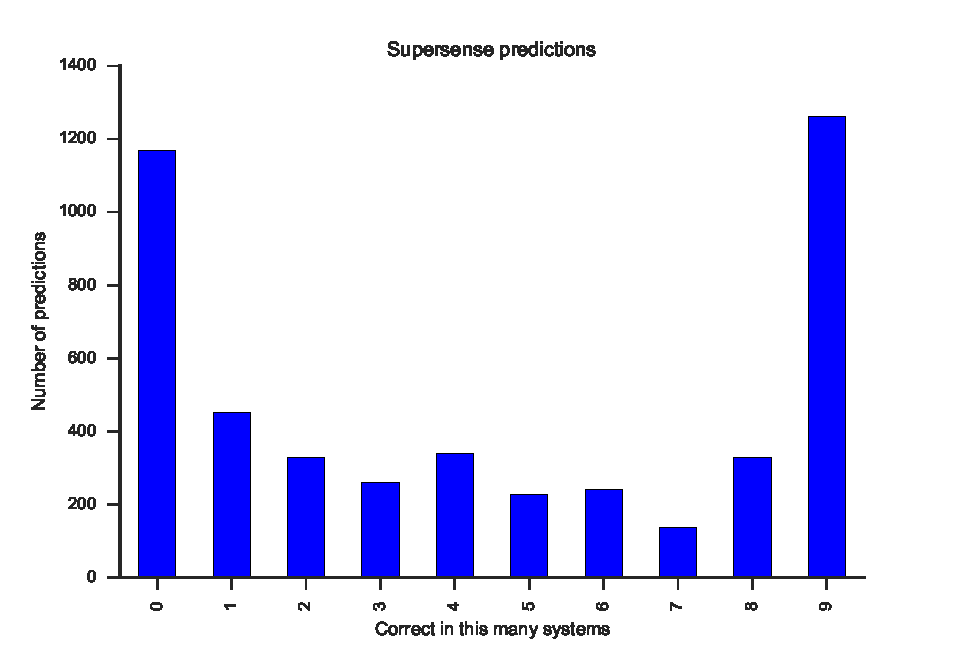
\includegraphics[width=8.5cm]{figs/supersense_predictions.pdf}
%	}
	\caption{Agreement in supersense decisions.}
	\label{fig:supersense-predictions}
\end{figure}

\begin{figure}
%	\resizebox{ \columnwidth }{!}{
		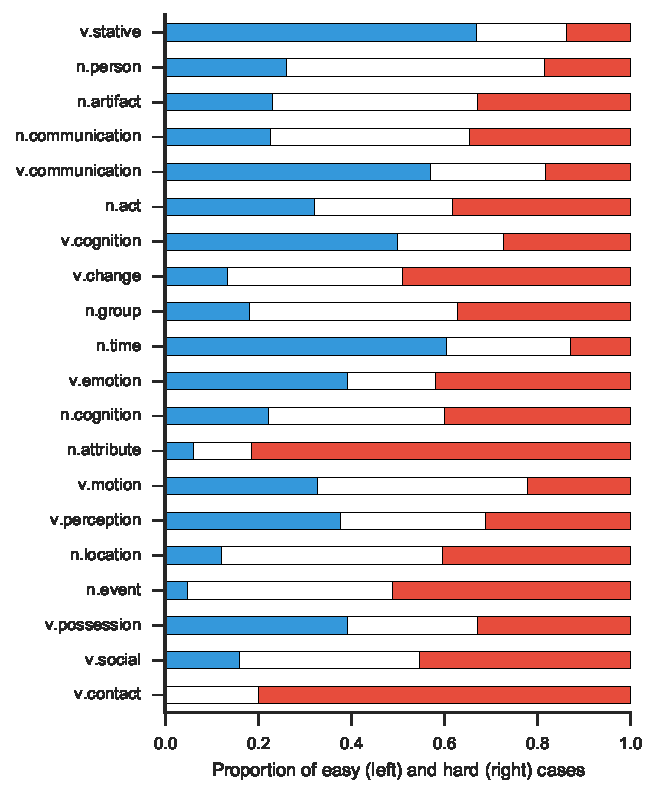
\includegraphics[width=8cm]{figs/proportion_of_easy_and_hard_supersenses.pdf}
%	}
	\caption{Easy and hard supersense decisions. Shown in blue in the left side of the plot is the proportion of instances of the given supersense type where at most one system gave the wrong answer. On the right side in red is the corresponding figure where at most one system gave the right answer.}
	\label{fig:easy-and-hard-supersenses}
\end{figure}


\subsection{Clusters of systems}

[To be filled in]

\begin{figure}
	\resizebox{ \columnwidth }{!}{
		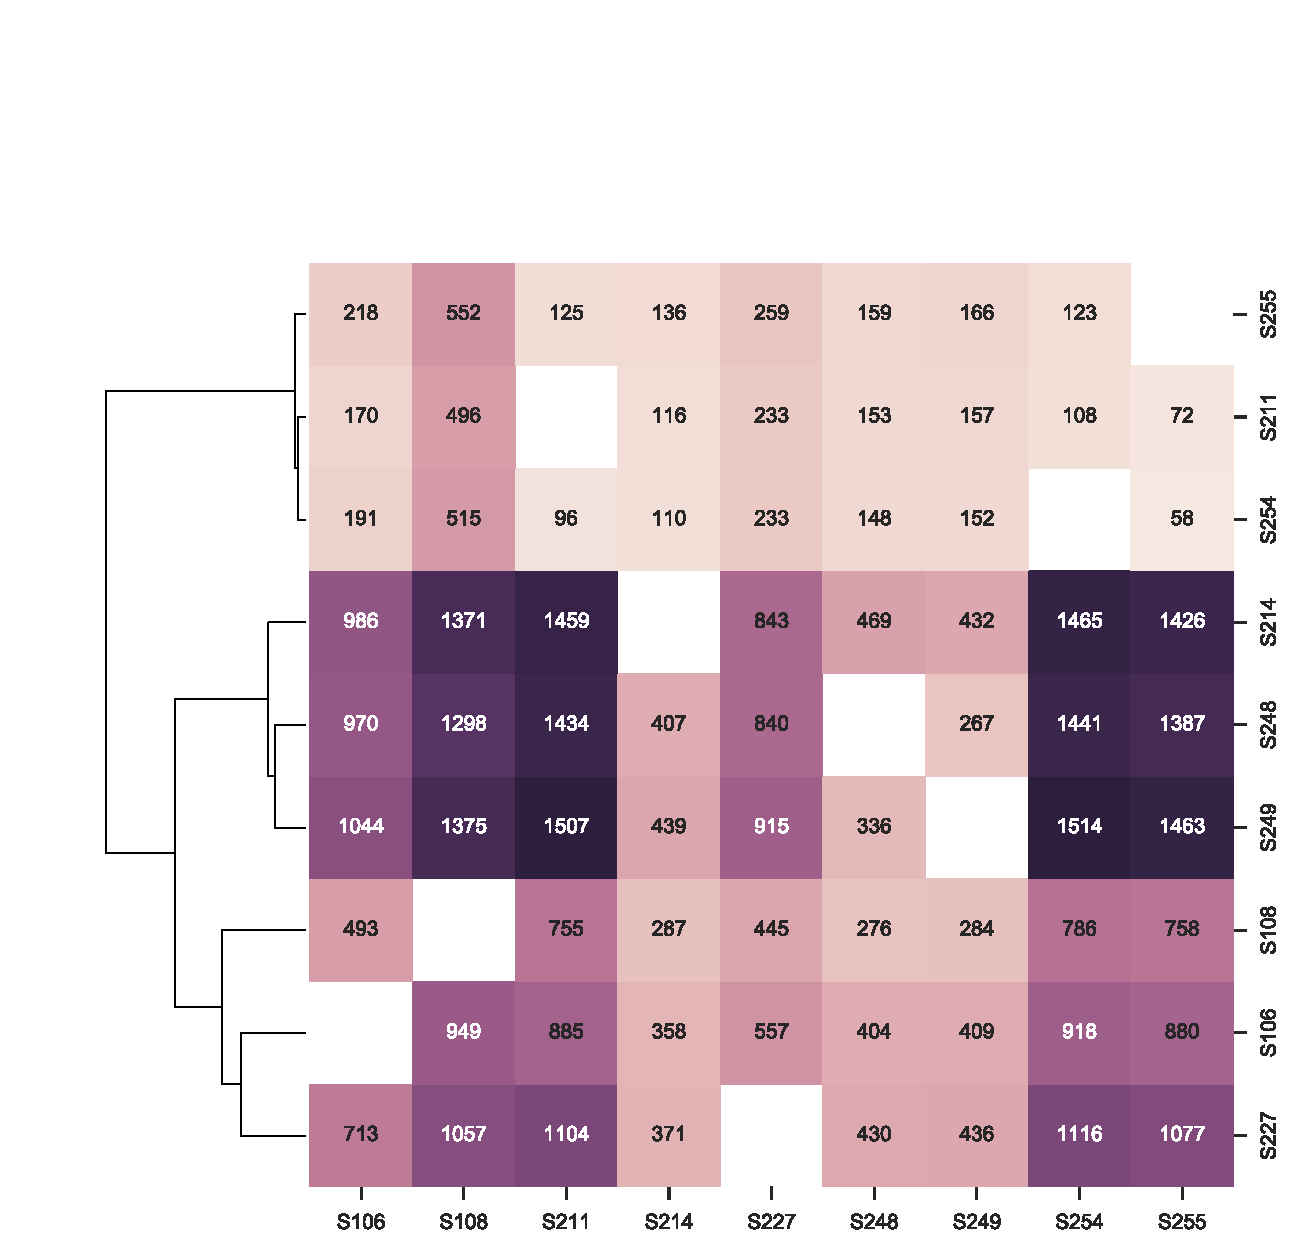
\includegraphics{figs/system_pairwise_clusters_cropped.pdf}
	}
	\caption{System clusters. Each cell compares the predictions of two systems $i$ and $j$ with respect to a gold standard. The value in the $i$,$j$-th cell is the number of predictions that $i$ got right but $j$ did not.}
	\label{fig:system-clusters}
\end{figure}


\begin{table}\small\centering
\begin{tabular}{lrrrr}
\toprule
{} &  Reviews &   TED &  Twitter &  All \\
submission &          &       &          &             \\
\midrule
\multicolumn{5}{l}{\textbf{Multiword expressions}} \\

106        &    49.6\% & 56.8\% &    51.2\% &       51.5\% \\
108        &    26.4\% & 33.4\% &    34.2\% &       31.0\% \\
211        &     9.1\% & 18.3\% &    15.8\% &       13.5\% \\
214        &    53.4\% & 57.1\% &    59.5\% &       56.7\% \\
227        &    36.2\% & 41.8\% &    39.3\% &       38.5\% \\
248        &    54.0\% & 52.3\% &    54.5\% &       53.9\% \\
249        &    54.8\% & 53.5\% &    61.1\% &       57.2\% \\
254        &     7.0\% & 16.3\% &     6.3\% &        8.2\% \\
255        &     8.7\% & 20.1\% &    15.5\% &       13.5\% \\[1.4ex]

\multicolumn{5}{l}{\textbf{Supersenses}} \\

106        &    50.9\% & 49.6\% &    49.2\% &       50.0\% \\
108        &    25.8\% & 24.7\% &    24.6\% &       25.1\% \\
211        &    52.0\% & 51.4\% &    50.0\% &       51.1\% \\
214        &    57.7\% & 60.1\% &    56.0\% &       57.6\% \\
227        &    51.4\% & 52.0\% &    51.7\% &       51.6\% \\
248        &    57.2\% & 59.1\% &    56.8\% &       57.5\% \\
249        &    57.0\% & 59.2\% &    57.5\% &       57.6\% \\
254        &    52.7\% & 51.4\% &    49.7\% &       51.3\% \\
255        &    52.0\% & 53.3\% &    51.1\% &       51.9\% \\[1.4ex]

\multicolumn{5}{l}{\textbf{Combined score}} \\

106        &    50.7\% & 50.6\% &    49.5\% &       50.2\% \\
108        &    25.9\% & 25.4\% &    25.9\% &       25.8\% \\
211        &    46.2\% & 47.9\% &    44.4\% &       45.9\% \\
214        &    57.0\% & 59.7\% &    56.6\% &       57.4\% \\
227        &    49.2\% & 50.8\% &    49.7\% &       49.8\% \\
248        &    56.7\% & 58.3\% &    56.4\% &       56.9\% \\
249        &    56.6\% & 58.3\% &    58.2\% &       57.6\% \\
254        &    46.6\% & 47.8\% &    43.0\% &       45.5\% \\
255        &    46.1\% & 49.8\% &    45.4\% &       46.6\% \\

\bottomrule
\end{tabular}

\caption{Per-domain evaluation results}	
\label{tbl:per-domain-results}
\end{table}





\section{Conclusion}
We propose a broad-coverage lexical semantic analysis task that combines MWE identification and supersense tagging. 
To guard against domain bias, we provide data sets from two different genres, namely online reviews and tweets. 
We expect that this task would draw participation from several subcommunities of NLP 
and that the resulting systems will contribute to a variety of applications.
%While the task is designed for English, we hope to extend it to other languages as well in future editions.









\begin{figure*}\small
\emph{Columns:} 1.~token offset (1-based); 2.~word token; 3.~lowercased lemma; 
4.~Universal POS tag; 5.~\textbf{MWE tag}; 6.~offset of nearest previous token 
in the same MWE, or \texttt{0} if not continuing an MWE (deterministic given column 5); 7.~(blank);
8.~\textbf{supersense label}, if any; 9.~sentence ID, including (at training time) the identity of the source corpus.
\begin{verbatim}
1       The          the        DET      O       0                                   ewtb.r.055976.1
2       staff        staff      NOUN     O       0               n.group             ewtb.r.055976.1
3       leaves       leave      VERB     B       0               v.cognition         ewtb.r.055976.1
4       a            a          DET      b       0                                   ewtb.r.055976.1
5       lot          lot        NOUN     i       4                                   ewtb.r.055976.1
6       to           to         PART     I       3                                   ewtb.r.055976.1
7       be           be         AUX      I       6                                   ewtb.r.055976.1
8       desired      desire     VERB     I       7                                   ewtb.r.055976.1
9       .            .          PUNCT    O       0                                   ewtb.r.055976.1

1       I            i          PRON     O       0                                   ewtb.r.329991.1
2       googled      google     VERB     O       0               v.communication     ewtb.r.329991.1
3       restaurants  restaurant NOUN     O       0               n.group             ewtb.r.329991.1
4       in           in         ADP      O       0                                   ewtb.r.329991.1
5       the          the        DET      O       0                                   ewtb.r.329991.1
6       area         area       NOUN     O       0               n.location          ewtb.r.329991.1
7       and          and        CONJ     O       0                                   ewtb.r.329991.1
8       Fuji         fuji       PROPN    B       0               n.group             ewtb.r.329991.1
9       Sushi        sushi      PROPN    I       8                                   ewtb.r.329991.1
10      came         come       VERB     B       0               v.communication     ewtb.r.329991.1
11      up           up         ADV      I       10                                  ewtb.r.329991.1
12      and          and        CONJ     O       0                                   ewtb.r.329991.1
13      reviews      review     NOUN     O       0               n.communication     ewtb.r.329991.1
14      were         be         VERB     O       0               v.stative           ewtb.r.329991.1
15      great        great      ADJ      O       0                                   ewtb.r.329991.1
16      so           so         ADV      O       0                                   ewtb.r.329991.1
17      I            i          PRON     O       0                                   ewtb.r.329991.1
18      made         make       VERB     B       0               v.communication     ewtb.r.329991.1
19      a            a          DET      o       0                                   ewtb.r.329991.1
20      carry        carry      VERB     b       0               v.possession        ewtb.r.329991.1
21      out          out        ADP      i       20                                  ewtb.r.329991.1
22      order        order      NOUN     I       18                                  ewtb.r.329991.1
23      of           of         ADP      O       0                                   ewtb.r.329991.1
24      :            :          PUNCT    O       0                                   ewtb.r.329991.1
25      L            l          SYM      O       0                                   ewtb.r.329991.1
26      17           17         NUM      O       0                                   ewtb.r.329991.1
27      .            .          PUNCT    O       0                                   ewtb.r.329991.1

1       Magic        magic      ADJ      B       0               n.group             lowlands-2
2       Key          key        NOUN     I       1                                   lowlands-2
3       Security     security   NOUN     I       2                                   lowlands-2
4       Locksmiths   locksmith  NOUN     I       3                                   lowlands-2
5       Save         save       ADJ      O       0                                   lowlands-2
6       ?            ?          PUNCT    O       0                                   lowlands-2
7       NUMBER       NUMBER     NUM      O       0               n.attribute         lowlands-2
8       on           on         ADP      O       0                                   lowlands-2
9       all          all        DET      O       0                                   lowlands-2
10      Booked       book       VERB     O       0               v.communication     lowlands-2
11      Services     services   NOUN     O       0               n.act               lowlands-2
12      with         with       ADP      O       0                                   lowlands-2
13      @USER        @USER      PROPN    O       0                                   lowlands-2
14      URL          URL        X        O       0                                   lowlands-2
15      @USER        @USER      PROPN    O       0                                   lowlands-2
\end{verbatim}
\caption{Column schema and example annotations in the 9-column tabular format.
There is one token per line; adjacent sentences are separated by a blank line.
In the sentence IDs, \texttt{ewtb.r} stands for the \textsc{Reviews} section of the English Web Treebank.}
\label{fig:tagsformat}
\end{figure*}

\bibliographystyle{style/aclnat}
% you bib file should really go here
\setlength{\bibsep}{10pt}
{\fontsize{10}{12.25}\selectfont
\bibliography{dimsum}}



\end{document}
